\begin{description}
\item[Speed of light] $2.998 * 10^8 m/s$
\item[Light year] $9.461 * 10^{15}$ m = 63 241 AU
\item[Observable Universe Boundary] $~14 * 10^9$ ly
\item[Average Earth-Moon distance] 385 000 km
\item[Average Earth-Sun distance (1 AU)] $1.4959 * 10^{11}$ m
\item[Diameter of the Sun] $1.391 * 10^6$ km
\item[Planck's constant (h)] $6.626 * 10^{-34} J \cdot s = 4.136 * 10^{-15} eV \cdot s$
\item[Stefan–Boltzmann constant] $5.67 * 10^{-8} \frac{W}{m^2 K^4}$
\item[Gravitational constant] $6.673 * 10^{-11} N \cdot (m/kg)^2$
\end{description}

\begin{center}
\scalebox{0.8}{
    \begin{tabular}{|p{2.5cm}|*{10}{c|}}
    \hline
    & Mercury & Venus & Earth & Moon & Mars & Jupiter & Saturn & Uranus & Neptune & Pluto \\
    \hline
    Mass ($10^{24}$ kg) &  0.330 &  4.87 &  5.97 &  0.073 &  0.642 &  1898 &  568 &  86.8 &  102 &  0.0131 \\ \hline
    Diameter (km) &  4879 &  12,104 &  12,756 &  3475 &  6792 &  142,984 &  120,536 &  51,118 &  49,528 &  2390 \\ \hline
    Density ($kg/m^3$) &  5427 &  5243 &  5514 &  3340 &  3933 &  1326 &  687 &  1271 &  1638 &  1830 \\ \hline
    Gravity ($m/s^2$) &  3.7 &  8.9 &  9.8 &  1.6 &  3.7 &  23.1 &  9.0 &  8.7 &  11.0 &  0.6 \\ \hline
    Escape Velocity (km/s) &  4.3 &  10.4 &  11.2 &  2.4 &  5.0 &  59.5 &  35.5 &  21.3 &  23.5 &  1.1 \\ \hline
    Rotation Period (hours) &  1407.6 &  -5832.5 &  23.9 &  655.7 &  24.6 &  9.9 &  10.7 &  -17.2 &  16.1 &  -153.3 \\ \hline
    Length of Day (hours) &  4222.6 &  2802.0 &  24.0 &  708.7 &  24.7 &  9.9 &  10.7 &  17.2 &  16.1 &  153.3 \\ \hline
    Distance from Sun ($10^6$ km) &  57.9 &  108.2 &  149.6 &  0.384* &  227.9 &  778.6 &  1433.5 &  2872.5 &  4495.1 &  5870.0 \\ \hline
    Perihelion ($10^6$ km) &  46.0 &  107.5 &  147.1 &  0.363* &  206.6 &  740.5 &  1352.6 &  2741.3 &  4444.5 &  4435.0 \\ \hline
    Aphelion ($10^6$ km) &  69.8 &  108.9 &  152.1 &  0.406* &  249.2 &  816.6 &  1514.5 &  3003.6 &  4545.7 &  7304.3 \\ \hline
    Orbital Period (days) &  88.0 &  224.7 &  365.2 &  27.3 &  687.0 &  4331 &  10,747 &  30,589 &  59,800 &  90,588 \\ \hline
    Orbital Velocity (km/s) &  47.4 &  35.0 &  29.8 &  1.0 &  24.1 &  13.1 &  9.7 &  6.8 &  5.4 &  4.7 \\ \hline
    Orbital Inclination (degrees) &  7.0 &  3.4 &  0.0 &  5.1 &  1.9 &  1.3 &  2.5 &  0.8 &  1.8 &  17.2 \\ \hline
    Orbital Eccentricity &  0.205 &  0.007 &  0.017 &  0.055 &  0.094 &  0.049 &  0.057 &  0.046 &  0.011 &  0.244 \\ \hline
    Axial Tilt (degrees) &  0.01 &  177.4 &  23.4 &  6.7 &  25.2 &  3.1 &  26.7 &  97.8 &  28.3 &  122.5 \\ \hline
    Mean Temperature (C) &  167 &  464** &  15 &  -20 &  -65 &  -110 &  -140 &  -195 &  -200 &  -225 \\ \hline
    Surface Pressure (bars) &  0 &  92 &  1 &  0 &  0.01 &  Unknown &  Unknown &  Unknown &  Unknown &  0 \\ \hline
    Number of Moons &  0 &  0 &  1 &  0 &  2 &  67 &  62 &  27 &  14 &  5 \\ \hline
    Ring System? &  No &  No &  No &  No &  No &  Yes &  Yes &  Yes &  Yes &  No \\ \hline
    Global Magnetic Field? &  Yes &  No &  Yes &  No &  No &  Yes &  Yes &  Yes &  Yes &  Unknown \\ \hline
    \end{tabular}
}
\end{center}
{\footnotesize * From the Earth}\\
{\footnotesize ** Due to intense greenhouse effect of thick atmosphere}\\

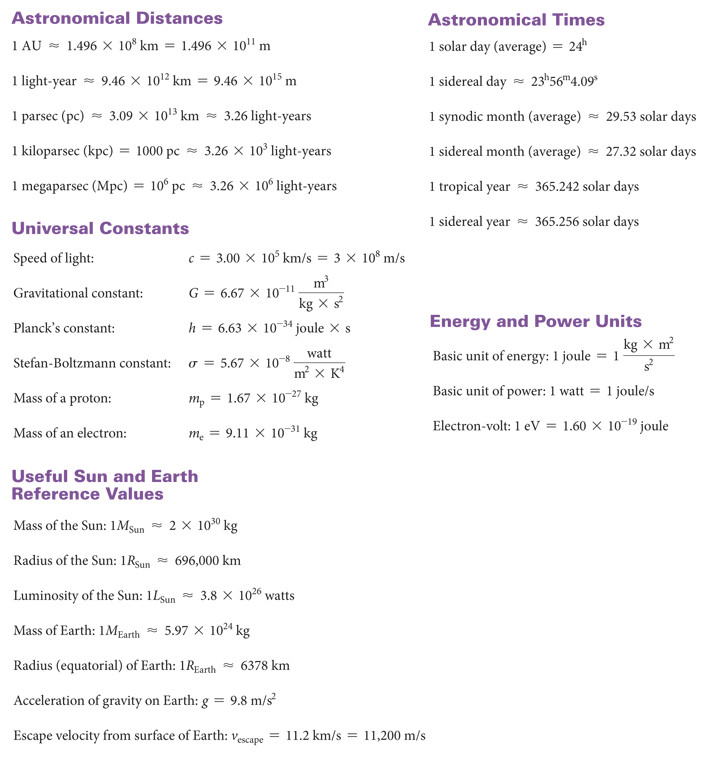
\includegraphics[scale=0.7]{constants}
